\chapter{Les differents paquetages}

\section{Relations entre les paquetages}
\par Nous avons �labor� huit paquetages d�finis ci-dessous :
\begin{itemize}
\item Identification : permet de g�rer les comptes.
\item Gestion des Sections : permet d'ajouter, de supprimer, de
modifier,(...) les noms de section tels Licence, maitrise ou DESS.
\item Gestion des Mati�res : permet d'ajouter, de supprimer, de
modifier,(...) les noms de mati�res tels Math�matiques, Genie logiciel ou base de donn�es.
\item Gestion des Enseignements : permet de g�rer les enseignements,
c'est � dire associer ou d�sassocier une ann�e avec des mati�res et
des sections.
\item Gestion des Devoirs : permet de manipuler des devoirs (projets ou TDs)
\item Gestion des Exercices : permet de manipuler des exercices :
(cr�ation suppression, modification ...)
\item Gestion des Corrections : permet de manipuler les corrections des exercices :
association et d�sassociation.
\item Gestion des FAQs :  permet de de g�rer la FAQ (ajout de question/r�ponse)
\end{itemize}


\begin{center}
\scalebox{0.5}{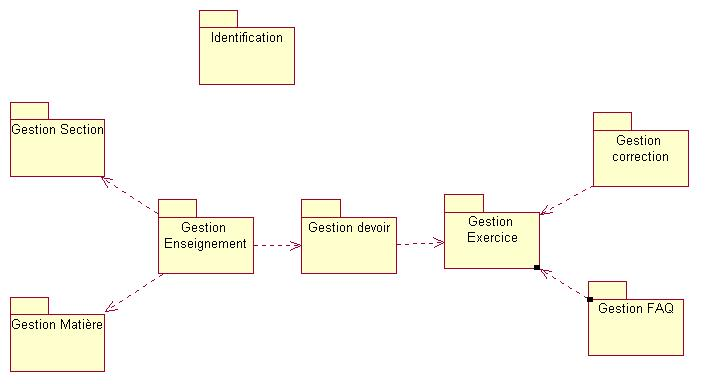
\includegraphics{images/main.jpg}}\\
\par{Relation entre les Paquetages} 
\end{center}
Nous allons maintenant expliciter les diff�rents paquetages.
